\section{Limites termodinâmicos para redistribuição de carbono}

% De fato, os resultados experimentais apresentados neste trabalho também são claramente discordantes com as considerações do modelo ERC, principalmente no que tange a ocorrência de reações competitivas.

Na Figura \ref{fig:ERC_chempot} é mostrado como os modelos ERC e ERC$\theta$ se comparam com os valores máximos de $w_C^\gamma$ medidos por DRX in situ. As curvas sólidas representam o potencial químico de carbono da martensita em função do teor de carbono na austenita calculados para 300, 375 e \SI{450}{\degreeCelsius}. O valor de $w_C^\gamma$ na condição ERC foi calculado para a temperatura de têmpera de \SI{170}{\degreeCelsius}. De forma similar à publicação original de Toji\cite{Toji2015}, a princípio os valores de $w_C^\gamma$ calculados pelo modelo ERC$\theta$ foram determinados assumindo a precipitação de orto e paracementita na martensita. Os teores de carbono na austenita calculados para os diferentes modelos são mostrados na Tabela \ref{tab:ERCtheta}.

\begin{table}
  \centering
  \caption{Comparação dos valores experimentais de teor de carbono na austenita (\% em massa) com os valores previstos pelos modelos ERC e ERC$\theta$ para dois carbonetos, orto e paracementita.}
  \begin{tabular}{ccccc}
    \hline
      Temperatura (\SI{}{\degreeCelsius}) & ERC ($T_T=$\SI{170}{\degreeCelsius}) & ERC$\theta$ orto & ERC$\theta$ para & Experimental \\
    \hline
      300 & 1,355 & 0,165 & 3,869 & 1,66 \\
      375 & 1,355 & 0,277 & 3,795 & 1,57 \\
      450 & 1,355 & 0,290 & 3,727 & 1,45 \\
    \hline
  \end{tabular}
  \label{tab:ERCtheta}
\end{table}

Em um primeiro momento é aparente que o modelo ERC descreve relativamente bem os valores experimentais. Entretanto, deve ser notado que de acordo com o modelo ERC o teor de carbono da martensita deve ter muito próximo de zero, uma vez que o modelo não considera a precipitação de carbonetos. Em relação ao modelo ERC$\theta$, quando a fase precipitada é a ortocementita o teor de carbono de na austenita é inferior à composição inicial da austenita (0,76\%). Ou seja, nessa situação, a etapa de partição causaria a difusão de carbono da austenita em direção à mistura de martensita e carbonetos. No caso da precipitação de paracementita, a condição ERC$\theta$ prevê valores muito maiores de $w_C^\gamma$ e, portanto, a partição de carbono da martensita para a austenita é termodinamicamente possível.

\begin{figure}
  \centering  
  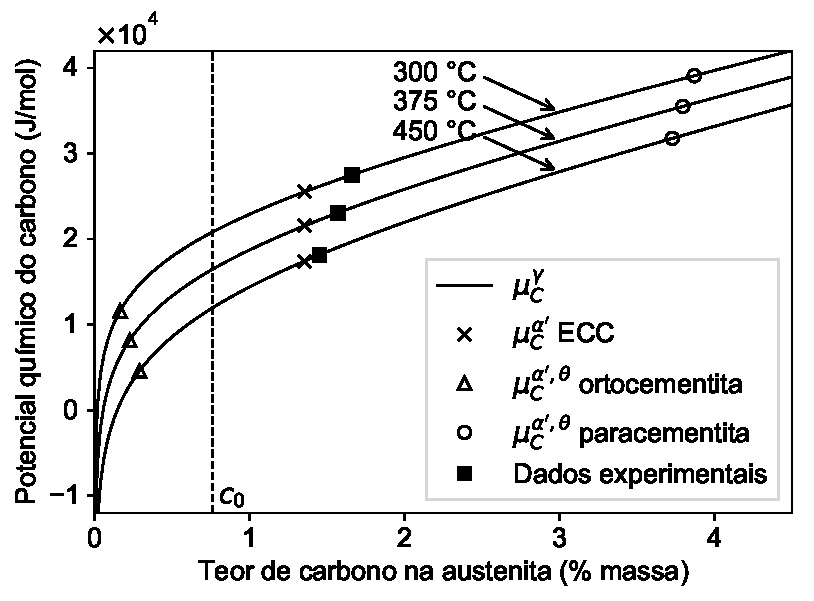
\includegraphics[width=.8\textwidth]{img/thermo-calc/CCE.pdf}
  \caption{Curvas de potencial químico de carbono $\mu_C^\gamma$ em função do teor de carbono na austenita. Os pontos dispersos representam os valores experimentais e aqueles calculados pelos modelos ERC e ERC$\theta$ (representados na Tabela \ref{tab:ERCtheta}).}
  \label{fig:ERC_chempot}
\end{figure}

Uma vez que a transformação incompleta da bainita claramente desempenha uma papel importante na redistribuição de carbono durante o processo T\&P, os resultados também foram analisados em torno dos limites termodinâmicos para reação bainítica. Os limites termodinâmicos para a reação bainítica ainda são razão de debate na literatura por dependerem do mecanismo aceito do crescimento da bainita. Se o mecanismo sem difusão é aceito, o limite termodinâmico para nucleação de novas subunidades de bainita é definido pela linha $T_0$, que corresponde ao par composição--temperatura em que as energias livres da ferrita e austenita são iguais. 
% A linha $T_0$ é por vezes modificada contabilizando a energia elástica associada à formação da bainita.
Por outro lado, se o mecanismo difusional é considerado, a reação bainítica deveria cessar uma vez que o equilíbrio metaestável entre ferrita e austenita é estabelecido. Uma vez que a reação bainítica acontece em temperaturas em que a partição de elementos substitucionais pode ser desprezada, o limite de paraequilíbrio entre ferrita e austenita é normalmente aceito. Entretanto, comumente a condição de paraequilíbrio não consegue descrever bem os limites da reação bainítica. Alternativamente, Hillert postulou a existência de uma energia adicional para o crescimento da ferrita bainítica e calculou tal energia a partir de um ajuste de dados experimentais. O limite termodinâmico resultante para crescimento de ferrita bainítica e ferrita de Widmanstätten é o então chamado \textit{WBs}. 

Na Figura \ref{fig:WBs_para} os valores experimentais de $w_C^\gamma$ são representandos sobre o diagrama de fases de paraequilíbrio da liga estudada e também comparados com as linhas $T_0$ e WBs. Os dados representados na Figura \ref{fig:WBs_para} também são apresentados na Tabela \ref{tab:WBs_para}. Os resultados experimentais são superestimados pela pela linha de paraequilíbrio $A_3^{para}$e subestimados pela curva $T_0$. Por outro lado, o modelo WBs descreve satisfatoriamente os valores experimentais. Para comparação, o carbono na austenita medido por difração de raios X convencional nas amostras austemperadas a 300 e \SI{375}{\degreeCelsius} por 2~h foram 1,60 e 1,63\%, respectivamente, e também coincidem bem com os dados do material T\&P e o limite WBs.

% criticize WBs? Hypothesize origin of thermodynamical barrier on transition carbides?

\begin{figure}
  \centering  
  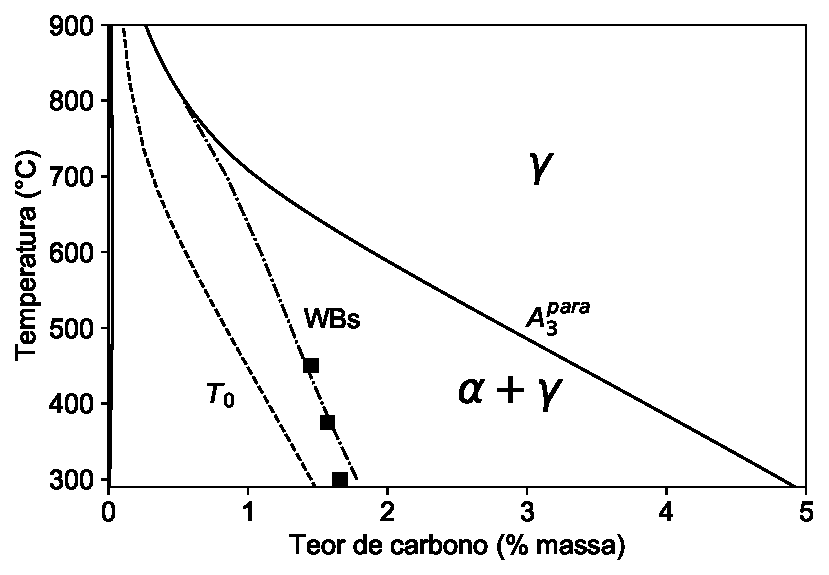
\includegraphics[width=.8\textwidth]{img/thermo-calc/WBs_para.pdf}
  \caption{Diagrama de fases de paraequilíbrio metaestável (apenas $\alpha$ e $\gamma$) calculado para a liga de ferro fundido. São representados diferentes limites termodinâmicos propostos para a reação bainítica: linha $A_3^{para}$, temperatura $T_0$ e o modelo WBs. Os pontos dispersos representam os dados experimentais de teor de carbono na austenita medidos por DRX in situ (dados representados na Tabela \ref{tab:WBs_para}).}
  \label{fig:WBs_para}
\end{figure}

\begin{table}
  \centering
  \caption{Comparação dos valores experimentais de teor de carbono na austenita (\% em massa) com os valores esperados por diferentes limites termodinâmicos propostos a reação bainítica: linha $A_3^{para}$, temperatura $T_0$ e a modelo WBs).}
  \begin{tabular}{ccccc}
    \hline
      Temperatura (\SI{}{\degreeCelsius}) & $A_3^{para}$ & WBs & $T_0$ & Experimental \\
    \hline
      300 & 4,824 & 1,780 & 1,451 & 1,66 \\
      375 & 4,095 & 1,590 & 1,223 & 1,57 \\
      450 & 3,353 & 1,417 & 0,992 & 1,45 \\
    \hline
  \end{tabular}
  \label{tab:WBs_para}
\end{table}